\documentclass{article}
\usepackage[margin=0.5in]{geometry}
\usepackage{xcolor}
\usepackage{tikz}
\usepackage{bm}
\usetikzlibrary{positioning,arrows.meta}

% =====================================================
% Three-color palette
% =====================================================
\definecolor{linegray}{RGB}{120,120,120}   % all strokes
\definecolor{fillblue}{RGB}{242,247,255}   % all fills

% =====================================================
% Global TikZ styles (single label size)
% =====================================================
\tikzset{
  arrow/.style={->, >=Latex, thick, draw=linegray},
  label/.style={font=\large, text=black},
  block/.style={
    draw=linegray,
    fill=fillblue,
    rectangle,
    rounded corners=2pt,
    minimum width=2.6cm,
    minimum height=2.0cm,
    align=center,
    font=\large
  },
  neuron/.style={
    circle,
    draw=linegray,
    fill=fillblue,
    thick,
    minimum size=1.2cm,
    inner sep=0pt
  }
}

\pagestyle{empty}
\begin{document}

% =====================================================
% Figure 1: Unrolled LSTM cells
% =====================================================
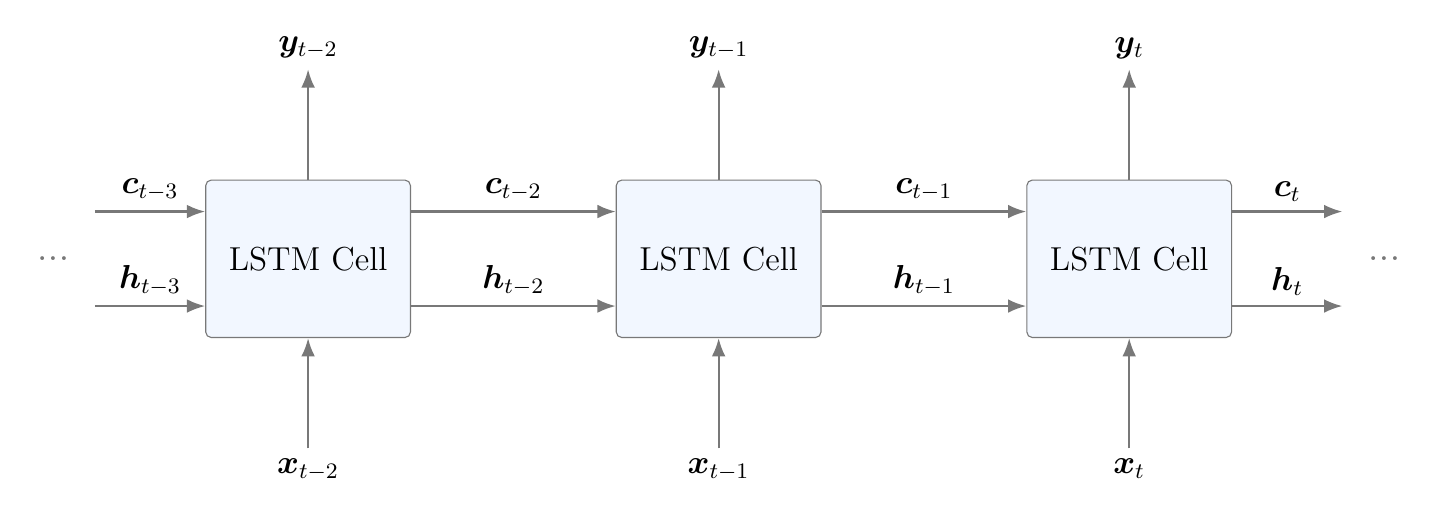
\begin{tikzpicture}[node distance=2.6cm]

\node[block] (c1) {LSTM Cell};
\node[block, right=of c1] (c2) {LSTM Cell};
\node[block, right=of c2] (c3) {LSTM Cell};

% Vertical inputs / outputs
\foreach \cell/\idx in {c1/{t-2}, c2/{t-1}, c3/t} {
  \draw[arrow] (\cell.south) ++(0,-1.4)
    node[below, label] {$\bm{x}_{\idx}$} -- (\cell.south);
  \draw[arrow] (\cell.north) -- ++(0,1.4)
    node[above, label] {$\bm{y}_{\idx}$};
}

\def\ys{0.6}

% Incoming states
\draw[arrow] ([yshift=\ys cm]c1.west) ++(-1.4,0) --
  ([yshift=\ys cm]c1.west)
  node[midway, above, label] {$\bm{c}_{t-3}$};

\draw[arrow] ([yshift=-\ys cm]c1.west) ++(-1.4,0) --
  ([yshift=-\ys cm]c1.west)
  node[midway, above, label] {$\bm{h}_{t-3}$};

\node[left=1.6cm of c1, font=\Large, text=linegray] {...};

% Between cells
\foreach \a/\b/\k in {c1/c2/{t-2}, c2/c3/{t-1}} {
  \draw[arrow] ([yshift=\ys cm]\a.east) -- ([yshift=\ys cm]\b.west)
    node[midway, above, label] {$\bm{c}_{\k}$};
  \draw[arrow] ([yshift=-\ys cm]\a.east) -- ([yshift=-\ys cm]\b.west)
    node[midway, above, label] {$\bm{h}_{\k}$};
}

% Outgoing states
\draw[arrow] ([yshift=\ys cm]c3.east) -- ++(1.4,0)
  node[midway, above, label] {$\bm{c}_{t}$};

\draw[arrow] ([yshift=-\ys cm]c3.east) -- ++(1.4,0)
  node[midway, above, label] {$\bm{h}_{t}$};

\node[right=1.6cm of c3, font=\Large, text=linegray] {...};

\end{tikzpicture}

\vspace{1cm}

% =====================================================
% Figure 2: RNN unrolling with U, W, V
% =====================================================
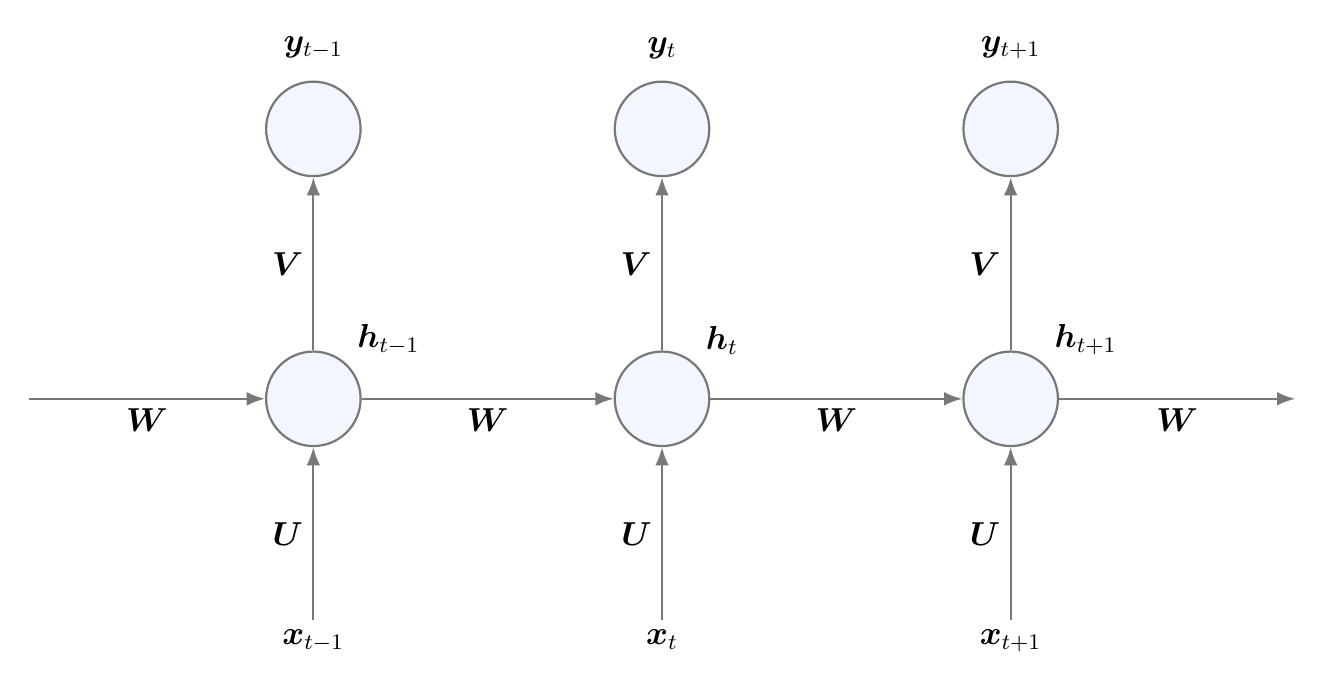
\begin{tikzpicture}[node distance=2.2cm and 3.2cm]

% Hidden states
\node[neuron] (ht) {};
\node[neuron, left=of ht] (htm1) {};
\node[neuron, right=of ht] (htp1) {};

% Outputs
\node[neuron, above=of ht] (yt) {};
\node[neuron, above=of htm1] (ytm1) {};
\node[neuron, above=of htp1] (ytp1) {};

% Inputs
\node[below=of ht, label] (xt) {$\bm{x}_t$};
\node[below=of htm1, label] (xtm1) {$\bm{x}_{t-1}$};
\node[below=of htp1, label] (xtp1) {$\bm{x}_{t+1}$};

% Labels
\node[above=0.15cm of yt, label] {$\bm{y}_t$};
\node[above=0.15cm of ytm1, label] {$\bm{y}_{t-1}$};
\node[above=0.15cm of ytp1, label] {$\bm{y}_{t+1}$};

\node[above right=0cm of ht, label] {$\bm{h}_t$};
\node[above right=0cm of htm1, label] {$\bm{h}_{t-1}$};
\node[above right=0cm of htp1, label] {$\bm{h}_{t+1}$};

% Connections: U
\draw[arrow] (xtm1) -- node[midway, left, label] {$\bm{U}$} (htm1);
\draw[arrow] (xt)   -- node[midway, left, label] {$\bm{U}$} (ht);
\draw[arrow] (xtp1) -- node[midway, left, label] {$\bm{U}$} (htp1);

% Connections: V
\draw[arrow] (htm1) -- node[midway, left, label] {$\bm{V}$} (ytm1);
\draw[arrow] (ht)   -- node[midway, left, label] {$\bm{V}$} (yt);
\draw[arrow] (htp1) -- node[midway, left, label] {$\bm{V}$} (ytp1);

% Recurrent W
\draw[arrow] (htm1) -- node[midway, below, label] {$\bm{W}$} (ht);
\draw[arrow] (ht)   -- node[midway, below, label] {$\bm{W}$} (htp1);

\draw[arrow] ([xshift=-3cm]htm1.west) --
  node[midway, below, label] {$\bm{W}$} (htm1);

\draw[arrow] (htp1) --
  node[midway, below, label] {$\bm{W}$} ([xshift=3cm]htp1.east);

\end{tikzpicture}




%%%%%%%%%%%%%%%%%%%%%%%%%%%%%%%


% Source - https://tex.stackexchange.com/a
% Posted by J Leon V., modified by community. See post 'Timeline' for change history
% Retrieved 2026-01-27, License - CC BY-SA 4.0
\usetikzlibrary{positioning, fit, arrows.meta, shapes}

% used to avoid putting the same thing several times...
% Command \empt{var1}{var2}
\newcommand{\empt}[2]{$#1^{\langle #2 \rangle}$}


\begin{tikzpicture}[
    % GLOBAL CFG
    font=\footnotesize,
    text=black,
    scale=1,
    every node/.style={transform shape},
    every label/.style={transform shape=false, font=\footnotesize},
    >=LaTeX,
    % Styles
    cell/.style={
        rectangle,
        rounded corners=5mm,
        draw=linegray,
        fill=fillblue,
        very thick,
    },
    operator/.style={
        circle,
        draw=linegray,
        fill=fillblue,
        thick,
        inner sep=-0.5pt,
        minimum height=.2cm,
    },
    function/.style={
        ellipse,
        draw=linegray,
        fill=fillblue,
        thick,
        inner sep=1pt
    },
    ct/.style={
        draw=none,
        inner sep=1pt
    },
    gt/.style={
        rectangle,
        draw=linegray,
        fill=fillblue,
        thick,
        minimum width=4mm,
        minimum height=3mm,
        inner sep=1pt
    },
    mylabel/.style={
        font=\footnotesize,
        text=black
    },
    ArrowC1/.style={
        rounded corners=.25cm,
        thick,
        draw=linegray,
    },
    ArrowC2/.style={
        rounded corners=.5cm,
        thick,
        draw=linegray,
    },
    peephole/.style={
        dashed,
        thick,
        draw=linegray,
    },
]

% =========================
% Main cell box
% =========================
\node [cell, minimum height=10cm, minimum width=14cm] at (0,0){} ;

% =========================
% Activation boxes (sig / tanh)
% =========================
\node [gt] (abox_f) at (-4,-1.5) {sig};
\node [gt] (abox_i) at (-3,-1.5) {sig};
\node [gt, minimum width=1cm] (abox_g) at (-1,-1.5) {tanh};
\node [gt] (abox_o) at (1,-1.5) {sig};

% Gate name labels above activation boxes
%\node[mylabel, above=2pt of abox_f] {$f_t$};
%\node[mylabel, above=2pt of abox_i] {$i_t$};
%\node[mylabel, above=2pt of abox_g] {$\tilde{c}_t$};
%\node[mylabel, above=2pt of abox_o] {$o_t$};

% Optional descriptive gate labels (vertical, like paper figures)
\node[mylabel, rotate=90] at (-4.2,-.4) {forget gate};
\node[mylabel, rotate=90] at (-3.2,-.4) {input gate};
\node[mylabel, rotate=90] at (-1.2,-.4) {new memory};
\node[mylabel, rotate=90] at (0.8, -.4 ) {output gate};

% =========================
% Operators / functions
% =========================
\node [operator] (mux_f) at (-4,3) {$\times$};   % f_t ⊙ c_{t-1}
\node [operator] (add_c) at (-1,3) {+};        % c_t sum
\node [operator] (mux_in) at (-1,1) {$\times$};  % i_t ⊙ c~_t
\node [operator] (mux_out) at (3,1) {$\times$};  % o_t ⊙ tanh(c_t)
\node [function] (tanh_c) at (3,2) {tanh};    % tanh(c_t)

% =========================
% External inputs (c_{t-1}, h_{t-1}, x_t)
% =========================
\node[ct, label={[mylabel]left:$c_{t-1}$}] (cprev) at (-8,3) {$c_{t-1}$};
\node[ct, label={[mylabel]left:$h_{t-1}$}] (hprev) at (-8,-3) {$h_{t-1}$};
\node[ct, label={[mylabel]below:$x_t$}]    (x)     at (-5,-6) {$x_t$};

% =========================
% External outputs (c_t, h_t, y_t)
% =========================
\node[ct, label={[mylabel]right:$c_t$}] (cnow) at (8,3) {$c_t$};
\node[ct, label={[mylabel]right:$h_t$}] (hnow) at (8,-3) {$h_t$};
\node[ct, label={[mylabel]above:$y_t$}] (y)    at (5,6)  {$y_t$};

% =========================
% Connections (kept from your template)
% =========================

% Top highway: c_{t-1} -> (×) -> (+) -> c_t
\draw [ArrowC1] (cprev) -- (mux_f) -- (add_c) -- (cnow);

% Inputs into activation boxes
\draw [ArrowC2] (hprev) -| (abox_o);
\draw [ArrowC1] (hprev -| abox_f)++(-1,0) -| (abox_f);
\draw [ArrowC1] (hprev -| abox_i)++(-1,0) -| (abox_i);
\draw [ArrowC1] (hprev -| abox_g)++(-1,0) -| (abox_g);
\draw [ArrowC1] (x) -- (x |- hprev) -| (abox_g);

% Peepholes (dashed) to gates (start inside cell, below sig boxes)
\coordinate (pf_start) at ([yshift=-0.6cm]abox_f.south);
\coordinate (pi_start) at ([yshift=-0.6cm]abox_i.south);
\coordinate (po_start) at ([yshift=-0.6cm]abox_o.south);
\path (cprev) -- (mux_f) coordinate[pos=0.65] (cprev_in);
\draw [peephole] (cprev_in) -| (pf_start);
\node[mylabel] at (-4.8,-2.8) {$p_f$};
\draw [peephole] (cprev_in) -| (pi_start);
\node[mylabel] at (-3.8,-2.8) {$p_i$};
\draw [peephole] (po_start) -| (cnow);
\node[mylabel] at (2.6,-2.8) {$p_o$};

% Internal gate-to-operator wiring
\draw [->, ArrowC2] (abox_f) -- (mux_f);     % f_t to mux_f
\draw [->, ArrowC2] (abox_i) |- (mux_in);    % i_t to mux_in
\draw [->, ArrowC2] (abox_g) -- (mux_in);    % c~_t to mux_in
\draw [->, ArrowC2] (abox_o) |- (mux_out);   % o_t to mux_out
\draw [->, ArrowC2] (mux_in) -- (add_c);     % i_t ⊙ c~_t to +
\draw [->, ArrowC1] (add_c -| tanh_c)++(-1,0) -| (tanh_c); % c_t to tanh
\draw [->, ArrowC2] (tanh_c) -- (mux_out);   % tanh(c_t) to mux_out

% Outputs: mux_out feeds h_t (and y_t from that branch)
\draw [-, ArrowC2] (mux_out) |- (hnow);

% y_t arrow from h_t branch (same structure you had)
\draw (cnow -| y) ++(0,-0.2) coordinate (i1);
\draw [-, ArrowC2] (hnow -| y)++(-1,0) -| (i1);
\draw [-, ArrowC2] (i1)++(0,0.4) -- (y);

\end{tikzpicture}


%%%%%%%%%%%%%%%%%%%%%%%%%%%%%










\end{document}
